\section{Yöntem}

[Bu bölümde araştırma deseni, veri toplama araçları, ölçekler, analiz adımları ve uygulama süreci açıklanmalıdır. Şablon dosyasındaki nota uygun olarak matematiksel model, gerekli yaklaşım ve örnek uygulama burada verilebilir.]

Bu çalışma kapsamında, tek şeritli bir yol üzerinde hareket eden otonom araçların güvenli ve verimli bir şekilde yönlendirilmesi için bir çizge yapısı üzerinde uzay-zaman  tabanlı bir rezervasyon modeli kurgulanmıştır. Problem, otonom araçların belirli depo noktalarından yük alıp başlangıca dönmesini hedeflerken; çarpışma, kilitlenme ve kapasite kısıtlarını aşmamayı amaçlayan bir çizelgeleme problemi olarak ele alınmıştır.

    \begin{figure}[h!]
    \centering
    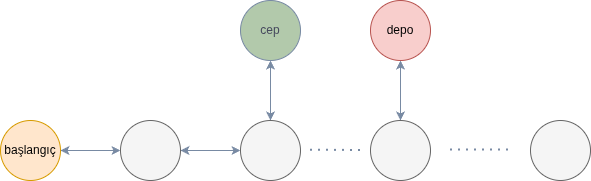
\includegraphics[width=0.7\linewidth]{img/graf-000.png}
    \caption{Genel Çizge Yapısı}
    \end{figure}

\subsection{Matematiksel Model}

Sistemin davranışını ve sınırlarını belirleyen matematiksel model; kümeler, karar değişkenleri ve kısıtlar üzerinden aşağıdaki şekilde tanımlanmıştır.

\subsubsection{Kümeler ve Parametreler} \label{sec:kümeler-ve-parametreler}

Yol uzunluğu $L = 240$ metredir.

\begin{itemize}
    \item $V = \{0, 10, 20, \dots, 240\}$: 10 metrelik adımlarla tanımlanmış yol düğümleri
    \item $C = \{80, 200\}$: Araçların bekleyebileceği cep düğümleri
    \item $G = \{70, 120, 240\}$: Araçların yük alabileceği depo düğümleri
    \item $S = \{0,40,80,120,160,200,240\}$: Her 40 metrede bir sensör bulunmaktadır.
    \item $A = \{1, 2, \dots, N\}$: Sistemdeki otonom araçlar ($3 \le N \le 20$)
    \item $T = \{0, 1, 2, \dots\}$: Ayrık zaman adımları
\end{itemize}

\subsubsection{Karar Değişkenleri}

t $\equiv$ zaman adımları olmak üzere $\forall t \in T$ olmaktadır. $x_i(t) \in V$: $i$-aracının $t$-anındaki konumunu ifade eder. $y_i$, $i$-aracının tüm görevlerini tamamlayıp başlangıç noktasına (0. metre) döndüğü anı temsil eder.

\subsubsection{Amaç Fonksiyonu (Makespan Minimizasyonu)}

Tüm araçların görevlerini tamamladığı toplam süreyi minimize etmek hedeflenmektedir:

\begin{equation}
    \min \max_{i \in A} y_i
\end{equation}

\subsubsection{Sistem Kısıtları} \label{sec:sistem-kısıtları}

\paragraph{Hareket Denklemi} Araçlar her adımda en fazla bir düğüm ilerleyebilir veya bekleyebilir.

\begin{equation}
    x_i(t+1) = x_i(t) + \Delta x, \quad \Delta x \in \{-10, 0, 10\}
\end{equation}

\paragraph{Güvenlik Mesafesi Kısıtı} İki araç arasındaki mesafe her zaman güvenli sınırlar içinde kalmalıdır. \textit{Bu kural cepler ve depolar dışındaki ana yolda mutlak geçerlidir.}

\begin{equation}
    \forall i \neq j, \forall t: |x_i(t) - x_j(t)| \ge d_{\text{min}} = 20 \text{ m}
\end{equation}
 
\paragraph{Kapasite Kısıtı} Herhangi bir $t$-anında bir cepte en fazla 1 araç, bir ara depoda ise en fazla 3 araç bulunabilir.

Bir diğer ifadeyle $\forall t$ için, $x \in C$ konumundaki araç sayısı $\le 1$. $x \in G$ araç sayısı $\le 3$ olmalıdır dolayısıyla:

Cepler için:

\begin{equation}
    \sum_{i \in A} \mathbf{1}(x_i(t) = c) \le 1, \quad \forall c \in C, \forall t \in T
\end{equation}

Depolar için:

\begin{equation}
    \sum_{i \in A} \mathbf{1}(x_i(t) = g) \le 3, \quad \forall g \in G, \forall t \in T
\end{equation}

biçiminde ifade edilebilir.

$\mathbf{1}(x_i(t) = c)$: Gösterme (Indicator) fonksiyonudur. Eğer araç o an $c$ konumundaysa $1$, değilse $0$ değerini alır.
 
\paragraph{Görev Kısıtı} Her araç, turunu tamamlamadan önce en az bir depoyu ziyaret etmelidir. Her araç turunu tamamladığında ($t = y_i$ anında), konumu $x_i(y_i) = 0$ olmalı ve $t < y_i$ için en az bir kez $x_i(t) \in G$ sağlanmalıdır.

\begin{equation}
    \exists t < y_i \text{ öyle ki } x_i(t) \in G \text{ ve } x_i(y_i) = 0
\end{equation}

\paragraph{Bekleme Eylemi Kısıtı} Bekleme eylemi yani herhangi bir aracın konumunu bir sonraki $t+1$ adımında değiştirmemesi ($x_i(t+1) = x_i(t)$), ancak bulunduğu konumun cepler ($C$), depolar ($G$) veya başlangıç ($0$) kümesinde olmasıyla mümkündür.

\begin{equation}
    (x_i(t+1) = x_i(t)) \implies x_i(t) \in C \cup G \cup \{0\}
\end{equation}

%%%%%%%%%%%%%%%%%%%%%%%%%%%

\subsection{Veri Yapıları ve Temsil}

Algoritmanın karmaşık kısıtlar altında çözüm üretebilmesi için yol ağı, araçlar ve zaman boyutu belirli veri yapıları kullanılarak soyutlanmıştır. Bu temsiller, A* algoritmasının durum uzayını verimli bir şekilde taramasına olanak tanır.

\subsubsection{Düğüm ve Çizge Yapısı}

Sistemdeki her bir fiziksel nokta, \texttt{(konum\_id, tür)} şeklinde bir üçlü demet olarak temsil edilir. Burada \texttt{konum\_id} aracın yol üzerindeki metresini (0-240), \texttt{tür} ise bulunduğu alanın fonksiyonunu (\texttt{yol}, \texttt{cep}, \texttt{depo}, \texttt{başlangıç}) belirtir. Bu ikili gösterim sayesinde, aynı koordinatta bulunan ancak farklı kapasite ve kurallara sahip olan \textit{ana yol} ve \textit{cep} düğümleri birbirinden ayrıştırılır. Çizge üzerindeki komşuluk ilişkileri, ana yol düğümlerinin birbirine doğrusal ($\pm$ 10m) bağlanması ve işlevsel düğümlerin (cep/depo) sadece kendi konumlarındaki yol düğümüne bağlanmasıyla kurulur.

\begin{figure}[h!]
    \centering
        \fbox{\rule{0pt}{4cm}\rule{0.7\linewidth}{0pt}}
%    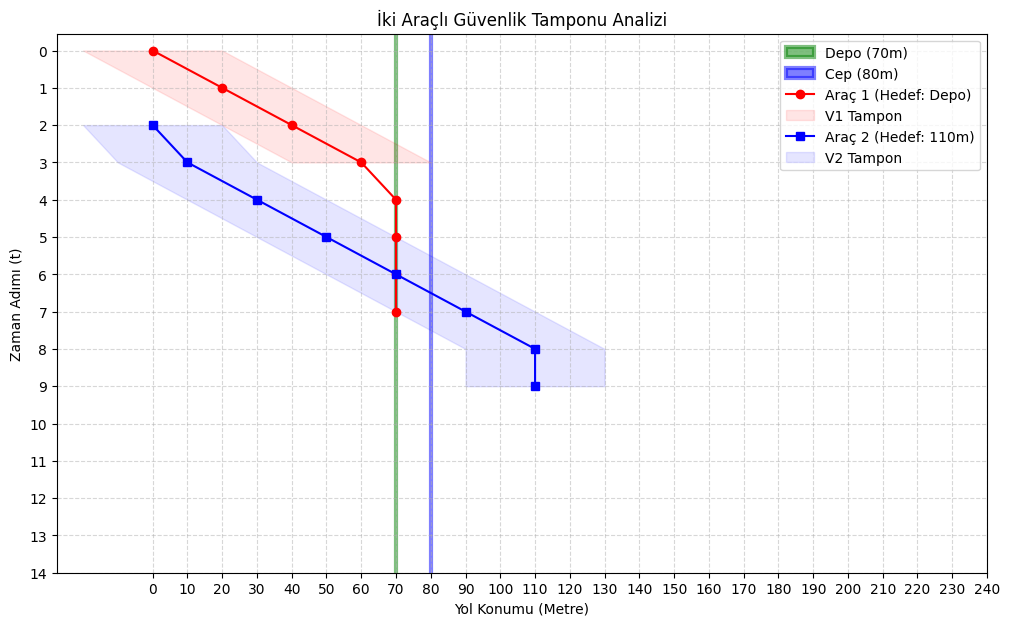
\includegraphics[width=0.9\linewidth]{img/uzay-zaman-grafiği-1.png}
    \caption{Çizge Yapısı Şekil Eklenecek}
    \label{fig:çizge-yapısı}
\end{figure}

Örneğin \texttt{(70, 'depo')} düğümü sadece \texttt{(70, 'yol')} düğümüne bağlı olurken \texttt{(70, 'yol')} düğümü \texttt{(60, 'yol')}, \texttt{(70, 'depo')} ve \texttt{(80, 'yol')} düğümlerine bağlı olacaktır. Aynı durum cep düğümleri için de geçerlidir.

Düğümler arası bağlantıları (Kenar Kümesi - $E$) veya komşuluk fonksiyonunu ($N(v)$) tanımlayabiliriz. Bir $(x, \tau)$ düğümünün komşuluk fonksiyonu $N(x, \tau)$ şu şekilde formüle edilebilir:

Ana yol düğümlerinin komşuları (hem yolda ileri/geri, hem de varsa bulunduğu konumdaki cep/depoya giriş):

\begin{equation}
    N(x, \text{'yol'}) = \{ (x \pm 10, \text{'yol'}) \} \cup \{ (x, \tau) \mid (x \in C \land \tau = \text{'cep'}) \lor (x \in G \land \tau = \text{'depo'}) \}
\end{equation}

Cep veya depo düğümlerinin komşuları (kendi içinde bekleme veya yola çıkma):

\begin{equation}
    N(x, \tau) = \{ (x, \tau), (x, \text{'yol'}) \} \quad \tau \in \{\text{'cep'}, \text{'depo'}\}
\end{equation}

\subsubsection{Durum Uzayı (State Space) Tanımı}

A* arama algoritması, sistemi statik bir harita yerine Zaman-Genişletilmiş Ağ (\textit{Time-Expanded Network}) üzerinde değerlendirir. Arama uzayındaki her bir durum, \texttt{(düğüm, zaman)} sıralı ikilisiyle tanımlanır. Bu yapı, aracın bir düğümde \textit{bekleme} eylemi yapmasını, zaman ($t \to t+1$) ilerlerken düğüm bilgisinin sabit kalması biçiminde modellemeyi sağlar. Arama, aracın başlangıç noktasındaki durumundan başlar ve hedef düğümün herhangi bir $t$-anındaki durumuna ulaşıldığında parça (\textit{segment}) bazlı olarak tamamlanır.

% Eleştiri: Zaman-Genişletilmiş Ağ (Time-Expanded Network) kavramı metinde çok iyi anlatılmış ama görseli yok. Sadece metinle 3B arama uzayını anlatmak okuyucuyu yorabilir.
% Öneri: Zamanın ($t$) dikey eksende, yol konumlarının yatay eksende olduğu, bir aracın "bekleme" eylemi yaptığında dikeyde nasıl sabit ilerlediğini gösteren basit bir Uzay-Zaman Grafiği çizip rapora eklemen, modelin anlaşılabilirliğini zirveye taşıyacaktır.

\begin{figure}[h!]
    \centering
%    \fbox{\rule{0pt}{4cm}\rule{0.7\linewidth}{0pt}}
    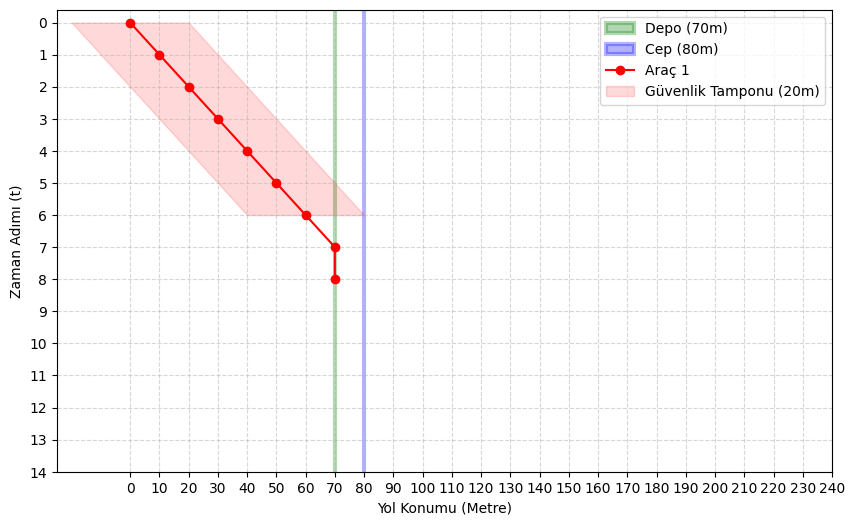
\includegraphics[width=0.9\linewidth]{img/uzay-zaman-grafiği-0.png}
    \caption{Güvenlik Tamponu ve Uzay-Zaman Grafiği}
    \label{fig:uzay-zaman-0}
\end{figure}


A* algoritmasının arama uzayı ($S$), fiziksel düğümler kümesi ($V$) ile zaman adımları kümesinin ($T$) Kartezyen çarpımıdır. Düğüm kümesi $V$ ise konumlar ($X$) ve tür ($\Gamma$) uzayının çarpımıdır.

\begin{equation}
    S = V \times T = \{ (x, \tau, t) \mid x \in X, \tau \in \Gamma, t \in T \}
\end{equation}

Burada $X = \{0, 10, \dots, 240\}$ ve $\Gamma = \{\text{yol, cep, depo, başlangıç}\}$ olarak düşünülebilir.

\autoref{fig:uzay-zaman-0}'deki senaryoda araç $x = 0$ ve $t = 0$ konumundan başlayarak sabit hızla $x=70$ konumundaki depoya ulaşmaktadır. Depoya girdiği andan itibaren güvenlik tamponu tahsisi kalkmaktadır.


\subsubsection{Merkezi Rezervasyon Tablosu ve Güvenlik Tamponu}

Araçlar arası çarpışmaları ve güvenlik mesafesi ihlallerini önlemek için merkezi bir rezervasyon veri yapısı kullanılmıştır. Bu yapı, \texttt{(konum, tür, zaman)} anahtarlarını karşılık gelen doluluk bilgisiyle eşleştiren bir sözlük (dictionary/hash map) olarak kurgulanmıştır. Bir araç için rota kesinleştiğinde, rotadaki her bir adım tabloya işlenir. Güvenlik mesafesi ($d_{min} = 20$) kuralını sağlamak adına, bir araç $t$-anında $x$-konumunda bulunuyorsa, tablodaki $x-20$, $x-10$, $x$, $x+10$, $x+20$ noktaları o zaman dilimi için rezerve edilerek diğer araçların bu bölgeye girmesi engellenir.

$i$-aracının $t$-anında oluşturduğu güvenlik tamponunu (rezerve edilen konumlar kümesi) $B_i(t)$ olarak tanımlarsak:

\begin{equation}
    B_i(t) = \{ x_i(t) + \delta \mid \delta \in \{-20, -10, 0, 10, 20\} \}
\end{equation}

Diğer araçların ($j \neq i$) çarpışma kısıtını sağlaması için rezervasyon tablosu gereği bu kümenin elemanı olmaması gerekir.


\begin{equation}
    x_j(t) \notin B_i(t), \quad \forall j \neq i
\end{equation}

\begin{figure}[h!]
    \centering
    %    \fbox{\rule{0pt}{4cm}\rule{0.7\linewidth}{0pt}}
    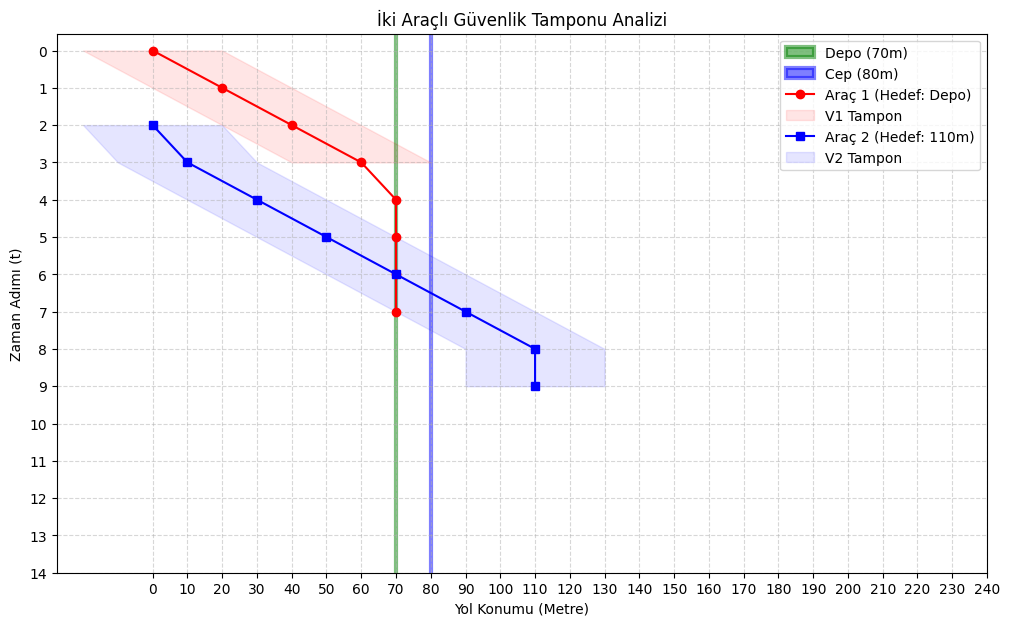
\includegraphics[width=0.9\linewidth]{img/uzay-zaman-grafiği-1.png}
    \caption{Güvenlik Tamponu ve Uzay-Zaman Grafiği}
    \label{fig:uzay-zaman-1}
\end{figure}

\autoref{fig:uzay-zaman-1}'deki senaryoda ilk araç $(0,0)$ konumundaki hareketi sonrasında $(70,t)$ konumundaki depoya ulaşmaktadır. İkinci araç ise güvenlik mesafesini koruyarak aracı takip ederek ilerelemektedir. Dikkat edilirse ilk araç depoya girdiğine güvenlik tamponu oluşmamaktadır. Öte yandan ikinci araç ise deponun konumundan geçerken güvenlik tamponu tahsis etmeye devam etmektedir. Bunun nedeni aracın depoya girmemesidir.

\subsubsection{Araç ve Görev Yönetimi}

Araçlar, kimlik bilgileri, öncelik durumları ve sıralı görev dizelgelerini içeren nesneler olarak tanımlanmıştır. Görevlerin parçalı yapısı (örneğin: 0 $\to$ \texttt{D70} $\to$ 0 $\to$ \texttt{D240} $\to$ 0), toplam yolculuğun segmentlere bölünmesini ve her segmentin bir önceki bitiş zamanını başlangıç kabul ederek ardışık olarak planlanmasını sağlar.

Bir $i$-aracının tüm görev rotasını ($M_i$), başlangıç noktasından (0) başlayıp aralarda $G$ kümesindeki depolara uğradığı ve sonunda yine başlangıca döndüğü sıralı n-demeti (ya da dizi) olarak ifade edebiliriz:

\begin{equation}
    M_i = \langle 0, g_{i,1}, 0, g_{i,2}, 0, \dots, g_{i,k}, 0 \rangle
\end{equation}

\begin{equation}
    \text{öyle ki } g_{i,m} \in G, \quad \forall m \in \{1, 2, \dots, k\}
\end{equation}

%%%%%%%%%%%%%%%%%%%%%%%%%%%%%%%%%

\subsection{Algoritma ve Çizelgeleme Yöntemi}

Problem, İşbirlikçi A* (\textit{Cooperative A*}) algoritması kullanılarak merkezi bir rezervasyon tablosu üzerinden çözülmektedir. Bu strateji, araçların birbirlerinin gelecek rotalarını bilerek hareket etmesini sağlar.

\subsubsection{Uzay-Zaman Rezervasyonu ve A* Taraması}

Her araç için rota planlaması yapılırken, 3 boyutlu bir durum uzayı (Konum $\times$ Tip $\times$ Zaman) taranır. Algoritma bir rota bulduğunda, bu rotadaki tüm konumları ve güvenlik tamponlarını (20m mesafe kuralı gereği komşu düğümleri) merkezi rezervasyon tablosuna işler. Böylece sonraki araçlar, planlarını yaparken önceden rezerve edilmiş bu alanlardan kaçınır.

\subsubsection{Maliyet Fonksiyonu} \label{sec:maliyet-fonksiyonu}

Algoritmanın araçları gereksiz manevralardan (\textit{yo-yo hareketi}) kaçındırması için asimetrik bir maliyet yapısı uygulanmıştır:

\begin{equation}
    c(s_t, s_{t+1}) = \begin{cases} 1.0, & \text{Eğer araç hareket ediyorsa} \\ 0.9, & \text{Eğer araç güvenli noktada (cep/depo/başlangıç) bekliyorsa} \end{cases}
\end{equation}

Bu düşük bekleme maliyeti, aracın yolu meşgul etmek yerine güvenli bir noktada durmasını teşvik eder. Böylece algoritma, hedefe yaklaşamayıp yolu uzatan çık-dön (\textit{yo-yo}) manevralarını $1.0 + 1.0 = 2.0$ maliyetle değerlendirirken, güvenli bir cepte/başlangıçta 2 birim beklemeyi $0.9 + 0.9 = 1.8$ maliyetle daha kârlı bulur ve gereksiz güzergahlar önlenir.

Maliyet fonksiyonu $c(s_t, s_{t+1})$, A* algoritmasının değerlendirme fonksiyonu olan $f(s) = g(s) + h(s)$ içerisinde başlangıçtan o anki duruma kadar olan kesin maliyeti ($g(s)$) hesaplamak için kullanılır:

\begin{equation}
    g(s_{t+1}) = g(s_t) + c(s_t, s_{t+1})
\end{equation}

Ayrıca algoritmanın hedef düğüme kalan tahmini mesafeyi hesapladığı sezgisel fonksiyon ($h(s)$), 1 boyutlu ağ üzerinde adım sayısı cinsinden \textit{Manhattan mesafesi} olarak tanımlanmıştır. Adım büyüklüğü $\Delta x = 10$ m olmak üzere:

\begin{equation}
    h(s_t) = \frac{|x(s_t) - x_{hedef}|}{\Delta x}
\end{equation}


\subsubsection{Araç İçi Görev Sıralaması (\textit{Local Task Sorting})} \label{sec:araç-içi-görev-sıralaması}

Algoritmanın genel performansını ve kilitlenme ihtimalini doğrudan etkileyen faktörlerden biri, her bir aracın kendi içindeki görevleri (ziyaret edeceği depoları) hangi sırayla gerçekleştirdiğidir. Bu çalışmada, araç içi görev sıralaması için En \textbf{Kısa İş İlk (\textit{Shortest Job First - SJF})} yaklaşımı kullanılmıştır. Bir araç birden fazla depoyu ziyaret edecekse, rotası başlangıç noktasına en yakın olan hedeften başlayacak şekilde sıralanır. Bu yöntemin temel amacı, araçların kısa mesafeli görevlerini hızla tamamlayıp ana yolu erken terk etmesini sağlamaktır. Ana yolun hızlı bir şekilde boşalması, diğer araçların hareket alanını genişleterek uzay-zaman tablosundaki rezervasyon çakışmalarını en aza indirir ve sistemin toplam tamamlanma süresini (\textit{makespan}) optimize eder.

Bir $i$-aracına atanmış sırasız hedef depolar kümesi $D_i \subseteq G$ olmak üzere, bu kümedeki elemanlar başlangıç noktasına (0. konum) olan mutlak uzaklıklarına göre küçükten büyüğe sıralanır. Bu işlem sonucunda $\langle g_{i,1}, g_{i,2}, \dots, g_{i,k} \rangle$ sıralı dizisi elde edilir ve sıralama kısıtı aşağıdaki eşitsizliği sağlar:

\begin{equation}
    |g_{i,1}| \le |g_{i,2}| \le \dots \le |g_{i,k}|
\end{equation}

Burada her bir $g_{i,m} \in D_i$, aracın sırayla gideceği depo konumudur. Otonom araçların her yük alımından sonra başlangıç noktasına dönme kuralı gereği, bu sıralı hedefler arasına 0. konum eklenerek aracın nihai parçalı rota dizisi ($M_i$) kurgulanır:

\begin{equation}
    M_i = \langle 0, g_{i,1}, 0, g_{i,2}, 0, \dots, g_{i,k}, 0 \rangle
\end{equation}


\subsubsection{Önceliklendirme ve Kilitlenme Çözümü} \label{sec:önceliklendirme-ve-kilitlenme-çözümü}

Sistemdeki araçlar, kilitlenmeleri (\textit{deadlock}) önlemek için belirli bir hiyerarşiye göre sırayla planlanır:

\begin{enumerate}
    \item \textbf{Özel Öncelik Durumu:} Öncelikli araçlar her zaman ilk sırada planlanır.
    \item \textbf{Fiziksel Konum Önceliği:} Tek şeritli yol hatlarında sollama imkanı olmadığından, yapay kilitlenmeleri önlemek adına hat üzerinde (0. metreden) daha ileride konumlanan araçlara öncelik verilerek öncelikle onların yolu boşaltması sağlanır.
    \item \textbf{Hedefe Yakınlık:} Mevcut hedefine daha yakın olan araçlara öncelik verilerek yolun öncelikle onlar tarafından boşaltılması sağlanır.
    \item \textbf{Gecikmeli Çıkış (\textit{Deadlock Resolver}):} Eğer bir araç için geçerli bir rota bulunamazsa, bu durum sistemin o anki yoğunluğu nedeniyle kilitlenmeye gittiğini gösterir. Çözüm olarak aracın yola çıkış zamanı ($t_{\text{başlangıç}}$) belirli bir adım kadar ötelenerek başlangıç noktasında bekletilir ve algoritma tekrar çalıştırılır. Bu mekanizma, yolda güvenli boşluklar oluşana kadar araçların sisteme girişini düzenleyerek yapay kilitlenmeleri (\textit{artificial deadlock}) engeller.
\end{enumerate}

Her $i$-aracı için çizelgeleme önceliği, üç bileşenli bir öncelik vektörü (\textit{tuple}) $\rho_i$ ile tanımlanmıştır. Algoritma bu vektörleri küçükten büyüğe değerlendirir.

Öncelik vektörünün bileşenleri şunlardır:

\begin{enumerate}
    \item $v_i \in \{0, 1\}$: Aracın özel öncelik durumu (öncelikli ise 1, değilse 0). Öncelikli araçların öne geçmesi için bu değer ters çevrilerek $(1 - v_i)$ olarak kullanılır.
    \item $-x_{\text{başlangıç}, i}$: Aracın yola çıktığı orijinal başlangıç noktası. Hat üzerinde daha ileride olan aracın küçük bir değer alarak öne geçmesi için bu değer negatif olarak eklenir.
    \item $d_i$: Aracın mevcut hedefine olan uzaklığı ($d_i = |x_{hedef} - x_i(t)|$).
    \item $W_i$: Aracın tüm görevleri boyunca kat edeceği toplam mesafe. Daha çok işi olan aracın öne geçmesi için bu değer negatif ($-W_i$) olarak vektöre eklenir.
\end{enumerate}

Buna göre $i$-aracının öncelik vektörü $\rho_i$ şu şekilde ifade edilir:

\begin{equation}
    \rho_i = (1 - v_i, -x_{\text{başlangıç}, i}, d_i, -W_i)
\end{equation}


Yalnızca hedefe olan uzaklığın ($d_i$) baz alınması, araçların farklı istasyonlara yöneldiği senaryolarda \textbf{yapay kilitlenmelere} yol açmaktadır. Örneğin; 20. ve 30. metrelerde konumlanan iki araçtan, 20. metredekinin hedefi Depo 70, 30. metredekinin hedefi ise Depo 120 olsun. Sadece hedefe yakınlık kriteri uygulandığında, 20. metredeki araç hedefine daha yakın olduğu için ($50 < 90$) ilk sırada çizelgelenmeye çalışılacaktır. Ancak tek şeritli hat üzerinde önünde bulunan 30. metredeki araç henüz hareket etmediği için $d_{\min}$ güvenlik tamponu anında ihlal edilecek ve kilitlenme oluşacaktır. Vektöre eklenen $-x_{\text{başlangıç}, i}$ bileşeni sayesinde, hat üzerinde fiziksel olarak daha önde olan (30. metredeki) araç ilk önce çizelgelenir; böylece güvenlik tamponunu arkasından gelen araç için temizleyerek yapay kilitlenmeyi engeller.

Problem kısıtları gereği, özel öncelikli araçlar daima başlangıç noktasında (0. metre) konumlanır ve tek bir görev (belirli bir depoya gidip dönme) üstlenirler. Algoritma bu araçları mutlak ilk sıraya alarak çizer. Bu kısıt, öncelikli araçların sistem henüz boşken rezerve edilmemiş bir uzay-zaman tablosunda ilerlemesini sağlar; böylece diğer araçların yaratabileceği yoğunluğa ve gecikmelere takılmadan, görevlerini matematiksel olarak mümkün olan en kısa sürede (optimal makespan ile) tamamlamaları garanti altına alınır.

İki araç karşılaştırıldığında sözlüksel sıralama (\textit{lexicographical order}) uygulanır. Eğer $\rho_i < \rho_j$ ise, $i$-aracı $j$-aracından önce çizelgelenir. Bu yapı sayesinde özel öncelikli araçlara mutlak üstünlük verilirken, eşitlik durumlarında sırasıyla hedefe yakınlık ve toplam iş yükü devreye girer.

\begin{figure}[h!]
    \centering
    %    \fbox{\rule{0pt}{4cm}\rule{0.7\linewidth}{0pt}}
    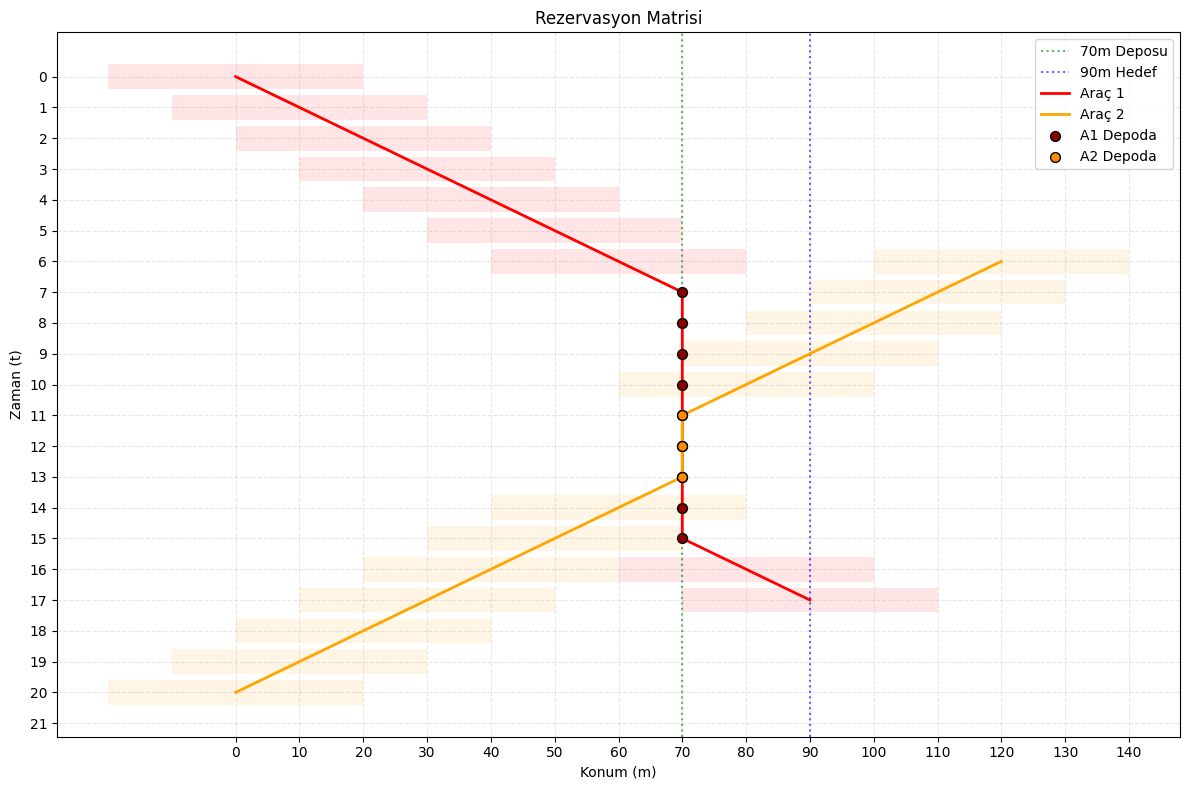
\includegraphics[width=0.9\linewidth]{img/uzay-zaman-grafiği-2.png}
    \caption{Yol Verme Senaryosu}
    \label{fig:uzay-zaman-2}
\end{figure}

\autoref{fig:uzay-zaman-2}'de daha önce çizelgelenmiş A2 aracı ve yol vermek için depoya giren A1 aracı bulunmaktadır. Bu örnekte A2 aracı depoya uğradıktan sonra depodan ayrılmakta ardından A1 aracı diğer aracın güvenlik tamponundan çıktıktan sonra depodan dışarı çıkmaktadır.

\subsubsection{Algoritma Karmaşıklığı}

% İşbirlikçi A* (CA*) algoritmasının hesaplama karmaşıklığı, arama yapılan durum uzayının (konum, tip, zaman) büyüklüğüne ve kullanılan veri yapılarına doğrudan bağlıdır. Algoritmanın performansını artıran en temel etmen, merkezi rezervasyon tablosunun bir Hash Map (sözlük) veri yapısı ile kurgulanmış olmasıdır. Bu sayede, A* algoritması yeni bir düğümü genişletirken yapması gereken $(x, \tau, t)$ durum çakışma (çarpışma ve kapasite) kontrollerini $O(1)$ sabit sürede gerçekleştirebilmektedir.

% Arama uzayının boyutu, fiziksel düğüm sayısı ($|V_{fiziksel}|$) ve algoritmanın ulaşabileceği maksimum zaman adımı ($T_{max}$) ile orantılıdır. Tek bir araç için en kötü durum zaman karmaşıklığı, 3 boyutlu graf üzerindeki standart A* davranışına paralel olarak $O(|V_{fiziksel}| \times T_{max} \log(|V_{fiziksel}| \times T_{max}))$ biçiminde ifade edilebilir. Toplam karmaşıklık ise $N$ adet araç için bu değerin araç sayısı ile çarpılmasıyla bulunur. Yoğun trafik senaryolarında, kilitlenme çözücü (\textit{deadlock resolver}) mekanizmasının devreye girmesi ve araçların yola çıkış zamanlarını ($t_{\text{başlangıç}}$) öteleyerek A* aramasını tekrar başlatması, algoritmik iş yükünü artıran (üstel büyümeye yaklaşan) bir faktördür. Ancak otonom araç yönlendirme problemlerinin doğası gereği, bu hesaplamalar araçlar yola çıkmadan önce çevrimdışı (offline) planlama aşamasında yapıldığından, elde edilen işlem süresi maliyeti sistemin kilitlenmeden güvenli çalışması adına kabul edilebilir bir düzeydedir.

İşbirlikçi A* algoritmasının zaman karmaşıklığı, fiziksel yol düğümlerinin ($V$) ve maksimum zaman adımının ($T_{max}$) oluşturduğu arama uzayına bağlıdır. Tek bir araç için en kötü durum (worst-case) zaman karmaşıklığı $O(|V| \times T_{max} \log(|V| \times T_{max}))$ olarak ifade edilebilir. Algoritmanın çalışma süresini asıl optimize eden unsur, merkezi rezervasyon tablosunun bir Hash Map (sözlük) veri yapısında kurgulanmasıdır. Bu sayede algoritmanın uzay-zaman tablosundaki çakışma ve güvenlik kontrolleri $O(1)$ sabit sürede yapılarak, dinamik araç sayısının yarattığı işlem yükü minimize edilmiştir.